\documentclass{article}
\usepackage[a4paper, margin=20mm]{geometry}
\usepackage{graphicx}
\usepackage{float}
\usepackage{amsmath}
\usepackage{amsfonts}
\usepackage{caption}
\usepackage{subcaption}

\title{Practical Submission Sheet}
\newcommand{\bb}[1]{\textbf{#1}}
%\newcommand{\it}[1]{\textit{#1}}
\newcommand{\ol}[1]{\overline{#1}}
\date{}
\begin{document}
	\maketitle
	
	\hrulefill
	\begin{center}
		\begin{tabular}{lll}
			\textit{Term}: 2020-1 & & \hfill \textit{Submission Date}: \today\\
			\textit{Lecture Date}: October 23, 2020. & & \textit{Practical Number}: 9\\
			\textit{Course Code}: PHY249 & & \textit{Section}: G2903\\
			\textit{Registration Number}: 11912610 & & \textit{Roll No}: 03\\
			\textit{Student Name}: Aayush Arya & & \\
		\end{tabular}
	\end{center}
	
	\hrulefill
	
	\section*{Aim} To design half-adder, full adder and 4-bit binary adder circuits using any gate combination.
	
	\section*{Concepts Learnt}	
	Learnt the implementation of binary adder circuits such as half, full and multi-bit (in this case, 4) adders.
	
	\section*{Key Observations \& Insights}
	The truth tables for all the circuits were verified. The boolean expressions for sum and carry in case of half adder are $S = A \oplus B $ and $C = A\cdot B$. For full adder, they are $S = (A \oplus B) \oplus C_{in}$ and $C_{out} = A\cdot B + (A\oplus B)\cdot C_{in}$
	
	\section*{Application Areas}
	Binary adders are used everywhere in digital electronics,  which is used in most modern electronic circuits in devices ranging from classical computers to internet of things devices (e.g. Arduino).
	
	\section*{Report}
	
	A half-adder circuit can be used to add two single bit numbers. It can be easily constructed using standard logic gates such as XOR and AND, as depicted in Figures 1-4. The rules for binary addition suggest that sum and carry are defined as $S = A \oplus B$ and $C = A\cdot B$ respectively.\\
	
	The truth table for these output functions is then
	\begin{table}[H]
		\centering
		\begin{tabular}{|c|c|c|c|}
			\hline
			Input A & Input B & Sum (S) & Carry (C)\\
			\hline
			0 & 0 & 0 & 0\\
			0 & 1 & 1 & 0\\
			1 & 0 & 1 & 0\\
			1 & 1 & 0 & 1\\
			\hline
		\end{tabular}
		\caption{Truth table for half-adder circuit.}
	\end{table}
	
	\begin{figure}[H]
		\centering
		\begin{subfigure}[t]{0.4\textwidth}
			\centering
			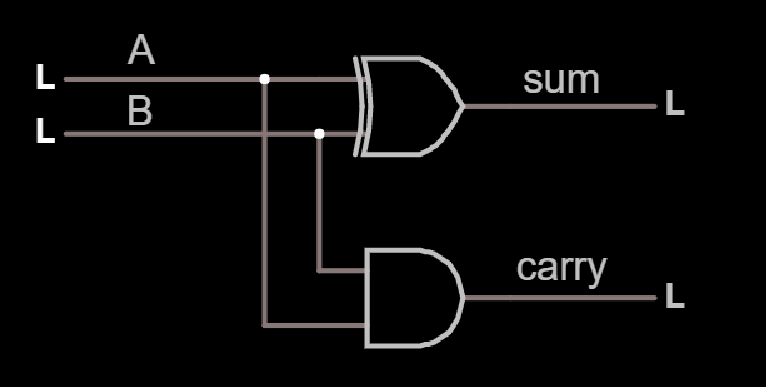
\includegraphics[width=\textwidth]{half_adder/half_adder_00}
			\caption{$A=0, B=0$}
		\end{subfigure}
		\begin{subfigure}[t]{.4\textwidth}
			\centering
			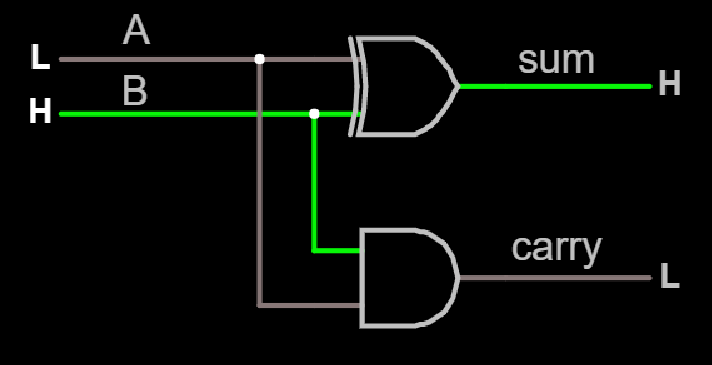
\includegraphics[width=\textwidth]{half_adder/half_adder_01.png}
			\caption{$A=0, B=1$}
		\end{subfigure}
		
		\begin{subfigure}[b]{0.4\textwidth}
			\centering
			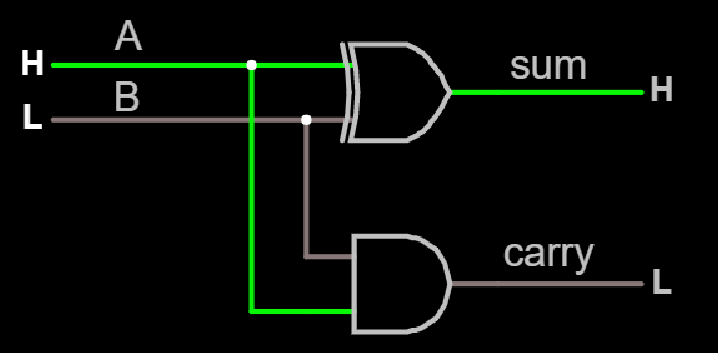
\includegraphics[width=\textwidth]{half_adder/half_adder_10.png}
			\caption{$A=1, B=0$}
		\end{subfigure}
		\begin{subfigure}[b]{0.4\textwidth}
			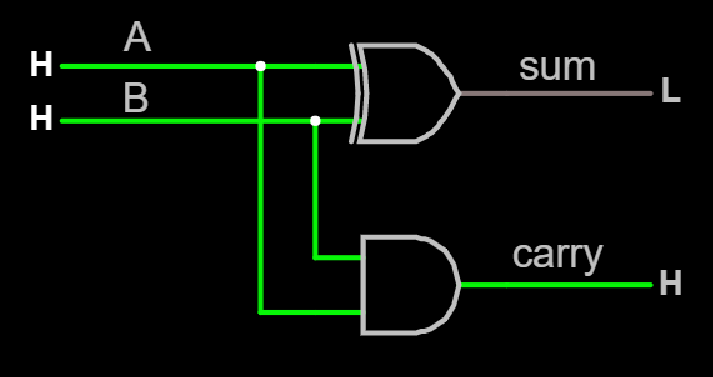
\includegraphics[width=\textwidth]{half_adder/half_adder_11.png}
			\caption{$A=1, B=1$}
		\end{subfigure}
		\caption{Different output states for a half-adder circuit}
		\label{fig:halfadder}
	\end{figure}
	
	The problem with a half-adder circuit is that, it can't deal with multi-bit numbers. One might want to input the carry of the sum of the rightmost two bits to another adder. For this, a \textit{full adder} circuit is used.
	
	Sum and carry for it are defined as $$S = (A \oplus B) \oplus C_{in}$$ and $$C_{out} = A\cdot B + (A\oplus B)\cdot C_{in}$$
	
	The truth table for it is
	\begin{table}[H]
		\centering
		\begin{tabular}{|c|c|c|c|c|}
			\hline
			Input A & Input B & C$_{in}$ & Sum (S) & Carry (C$_{out}$)\\
			\hline 
			0 & 0 & 0 & 0 & 0\\
			0 & 1 & 0 & 1 & 0\\
			1 & 0 & 0 & 1 & 0\\
			1 & 1 & 0 & 0 & 1\\
			\hline
			0 & 0 & 1 & 1 & 0\\
			0 & 1 & 1 & 0 & 1\\
			1 & 0 & 1 & 0 & 1\\
			1 & 1 & 1 & 1 & 1\\
			\hline
		\end{tabular}
		\caption{Truth table for full adder.}
	\end{table}
	
	The circuit for a full adder was constructed based on the boolean expressions for $S$ and $C_{out}$ and its different states are shown in Figure 2.
	
	\begin{figure}[H]
		\centering
		\begin{subfigure}[t]{0.4\textwidth}
			\centering
			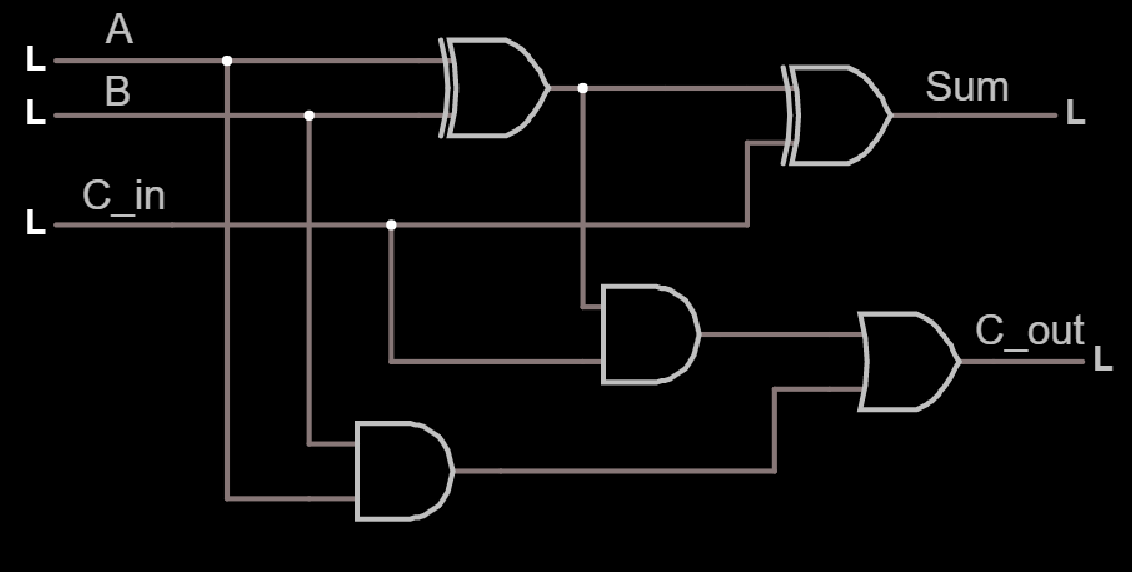
\includegraphics[width=\textwidth]{full_adder/full_adder_000.png}
		\end{subfigure}
		\begin{subfigure}[t]{.4\textwidth}
			\centering
			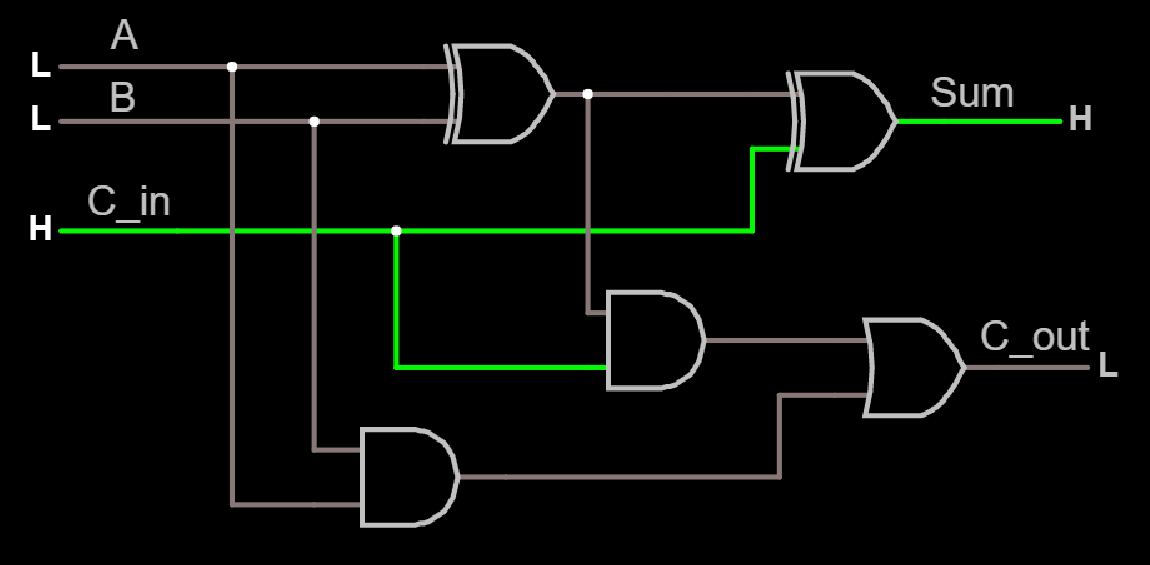
\includegraphics[width=\textwidth]{full_adder/full_adder_001.png}
		\end{subfigure}
		
		\begin{subfigure}[b]{0.4\textwidth}
			\centering
			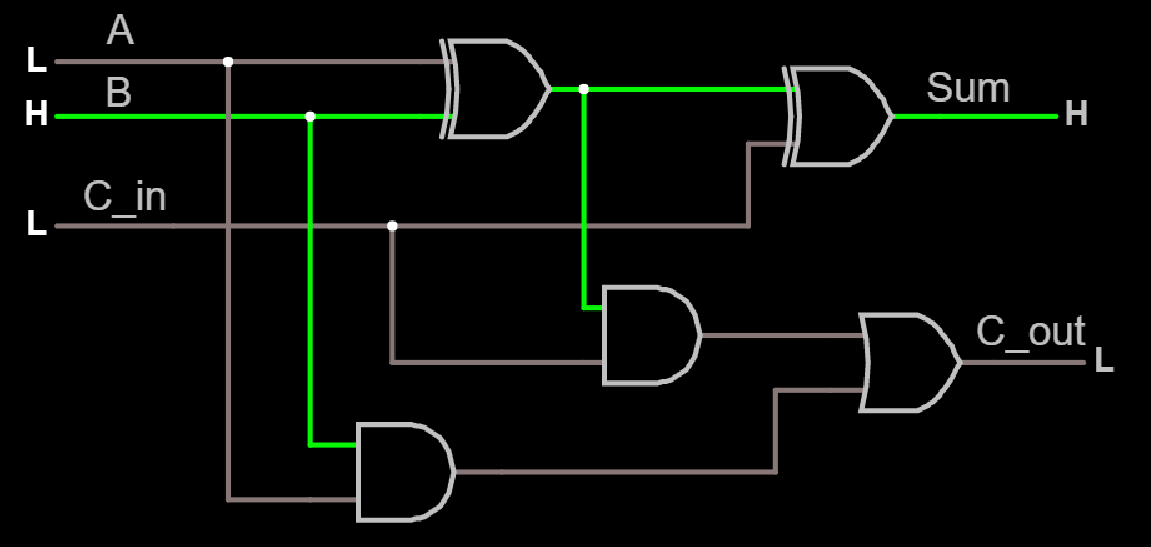
\includegraphics[width=\textwidth]{full_adder/full_adder_010.png}
		\end{subfigure}
		\begin{subfigure}[b]{0.4\textwidth}
			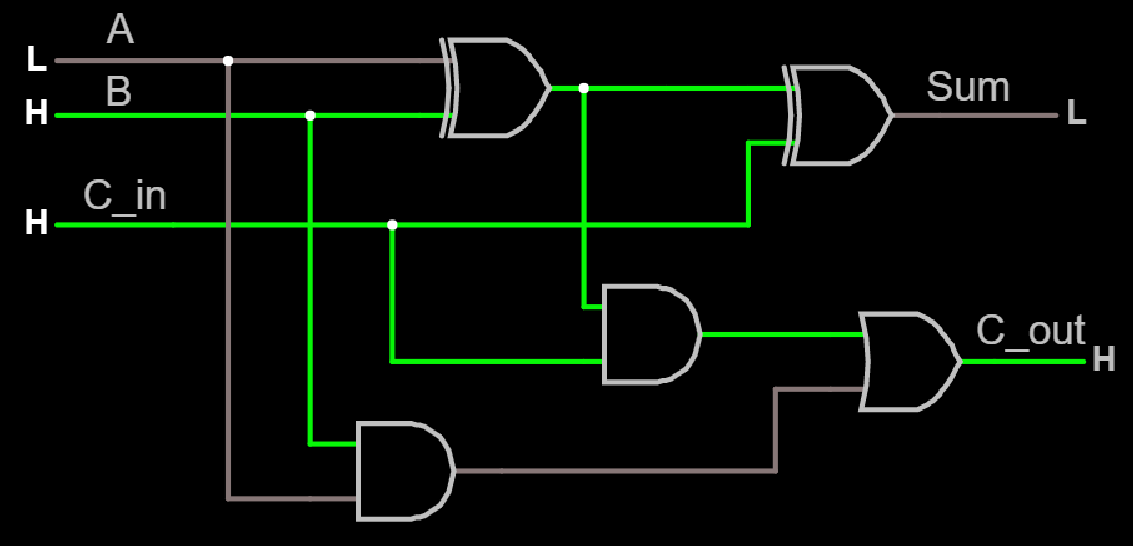
\includegraphics[width=\textwidth]{full_adder/full_adder_011.png}
		\end{subfigure}
		
		\begin{subfigure}[b]{0.4\textwidth}
			\centering
			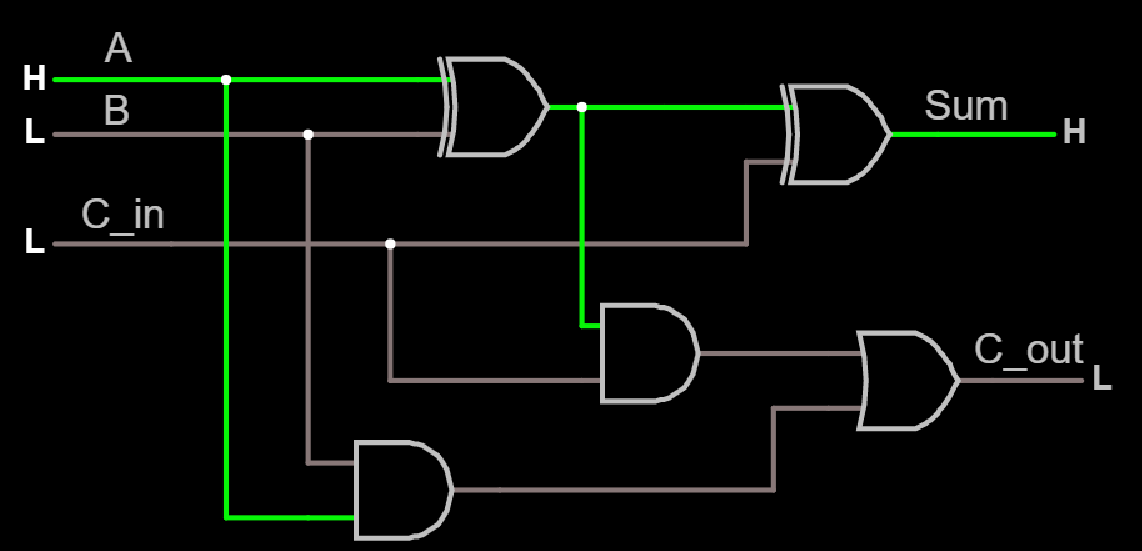
\includegraphics[width=\textwidth]{full_adder/full_adder_100.png}
		\end{subfigure}
		\begin{subfigure}[b]{0.4\textwidth}
			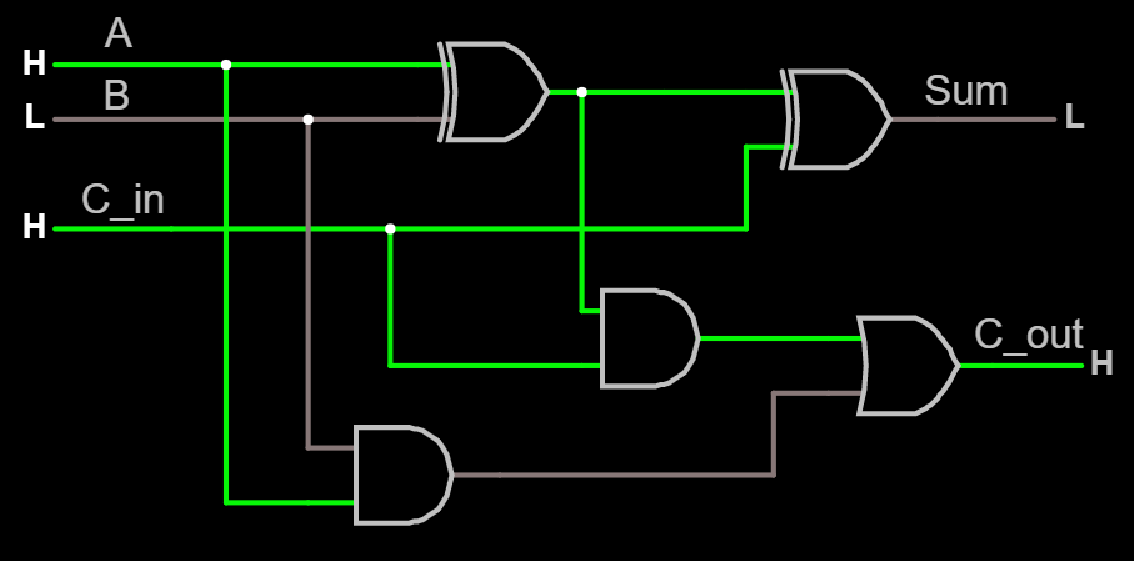
\includegraphics[width=\textwidth]{full_adder/full_adder_101.png}
		\end{subfigure}
		
		\begin{subfigure}[b]{0.4\textwidth}
			\centering
			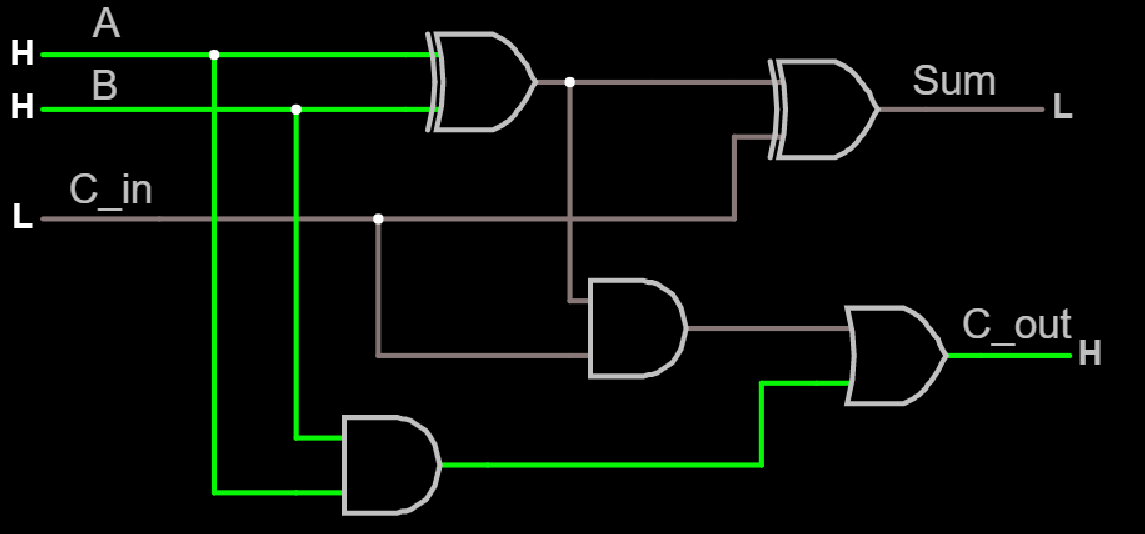
\includegraphics[width=\textwidth]{full_adder/full_adder_110.png}
		\end{subfigure}
		\begin{subfigure}[b]{0.4\textwidth}
			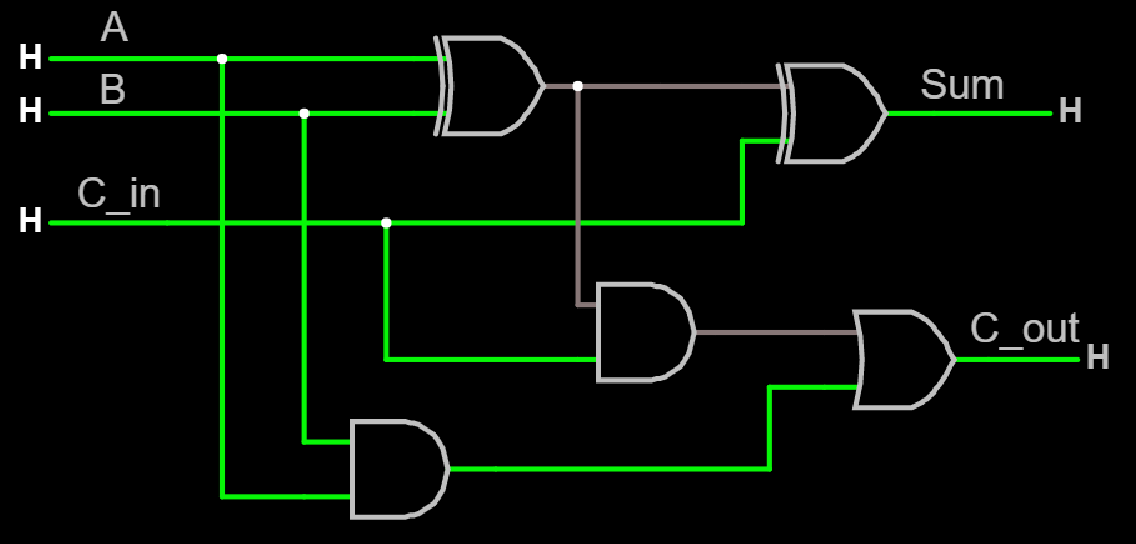
\includegraphics[width=\textwidth]{full_adder/full_adder_111.png}
		\end{subfigure}
		\caption{Different output states for a full-adder circuit}
		\label{fig:fulladder}
	\end{figure}
	
	Using combinations of full adder circuits, adders of multi-bit numbers can be constructed. The construction for 4 bit binary adder is shown in Figures 3 and 4.
	
	\begin{figure}[H]
		\centering
		\begin{subfigure}[t]{0.8\textwidth}
			\centering
			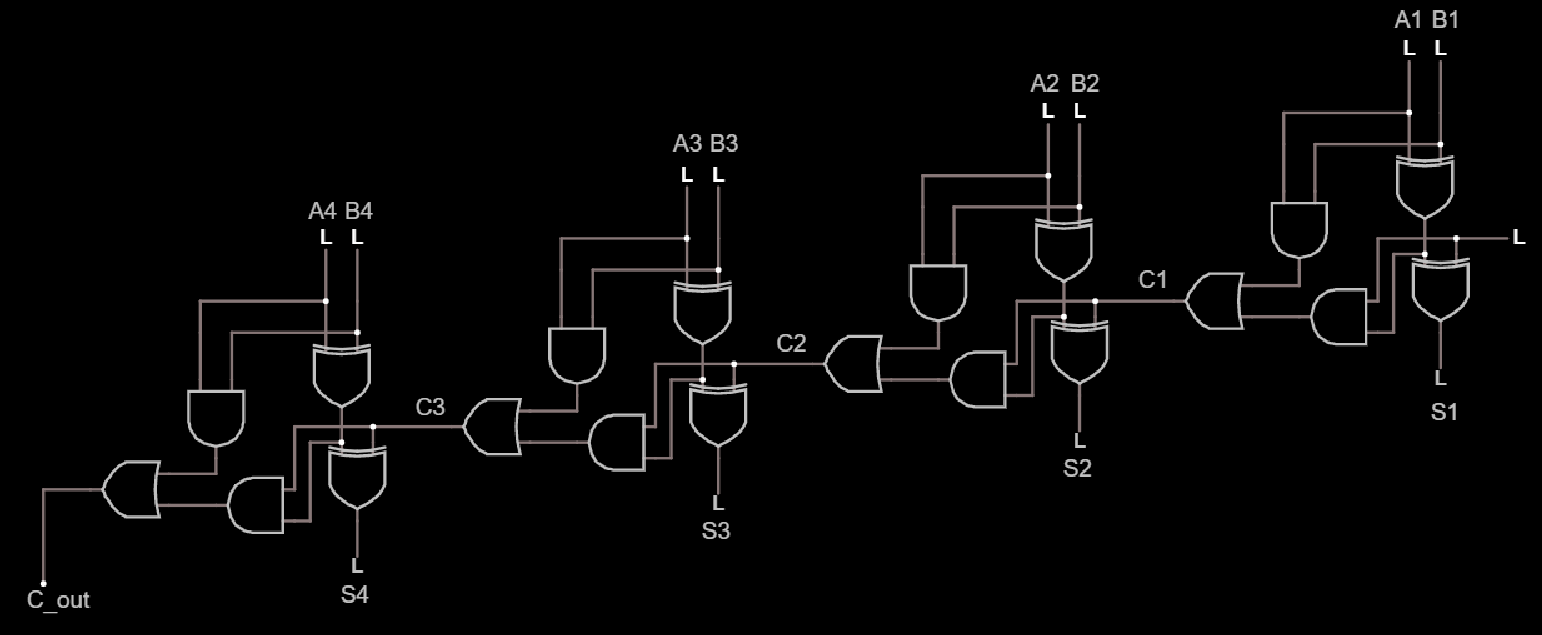
\includegraphics[width=\textwidth]{4bit/4bit_000.png}
		\end{subfigure}
		
		\begin{subfigure}[b]{0.8\textwidth}
			\centering
			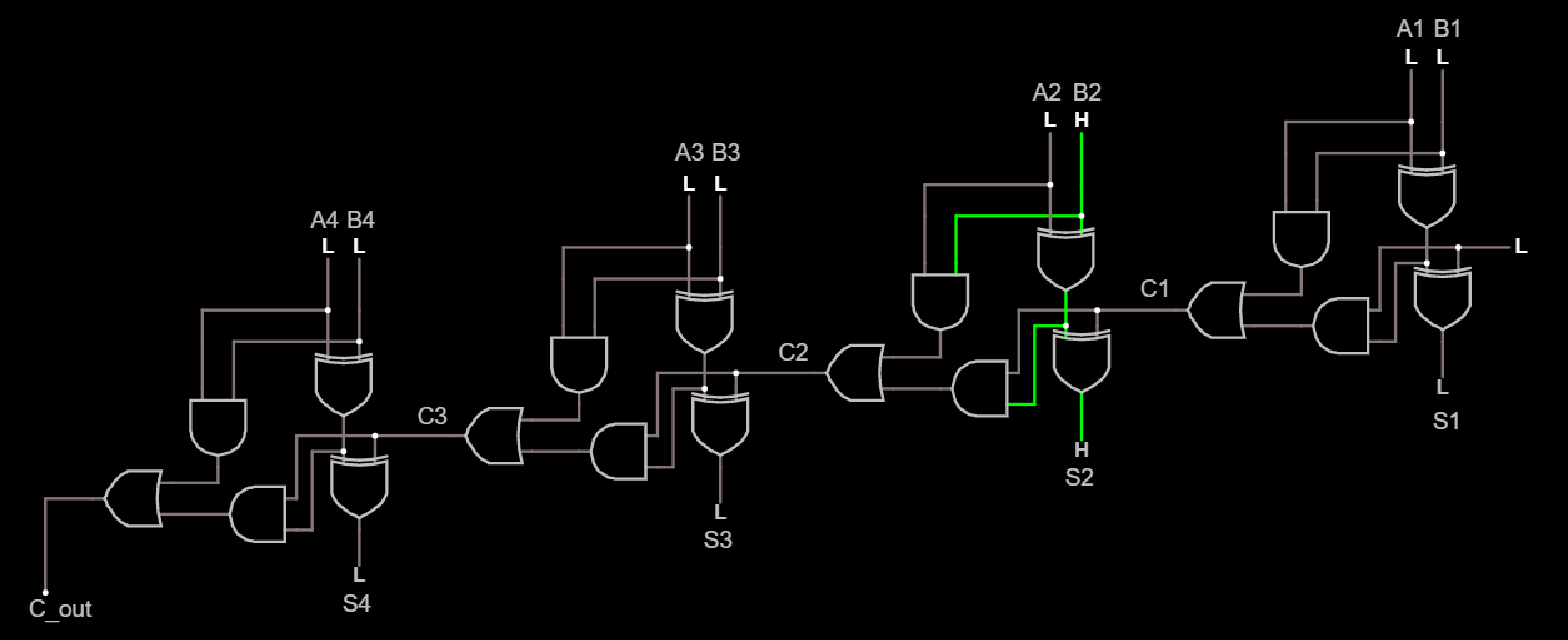
\includegraphics[width=\textwidth]{4bit/4bit_010.png}
		\end{subfigure}
		
		\begin{subfigure}[b]{0.8\textwidth}
			\centering
			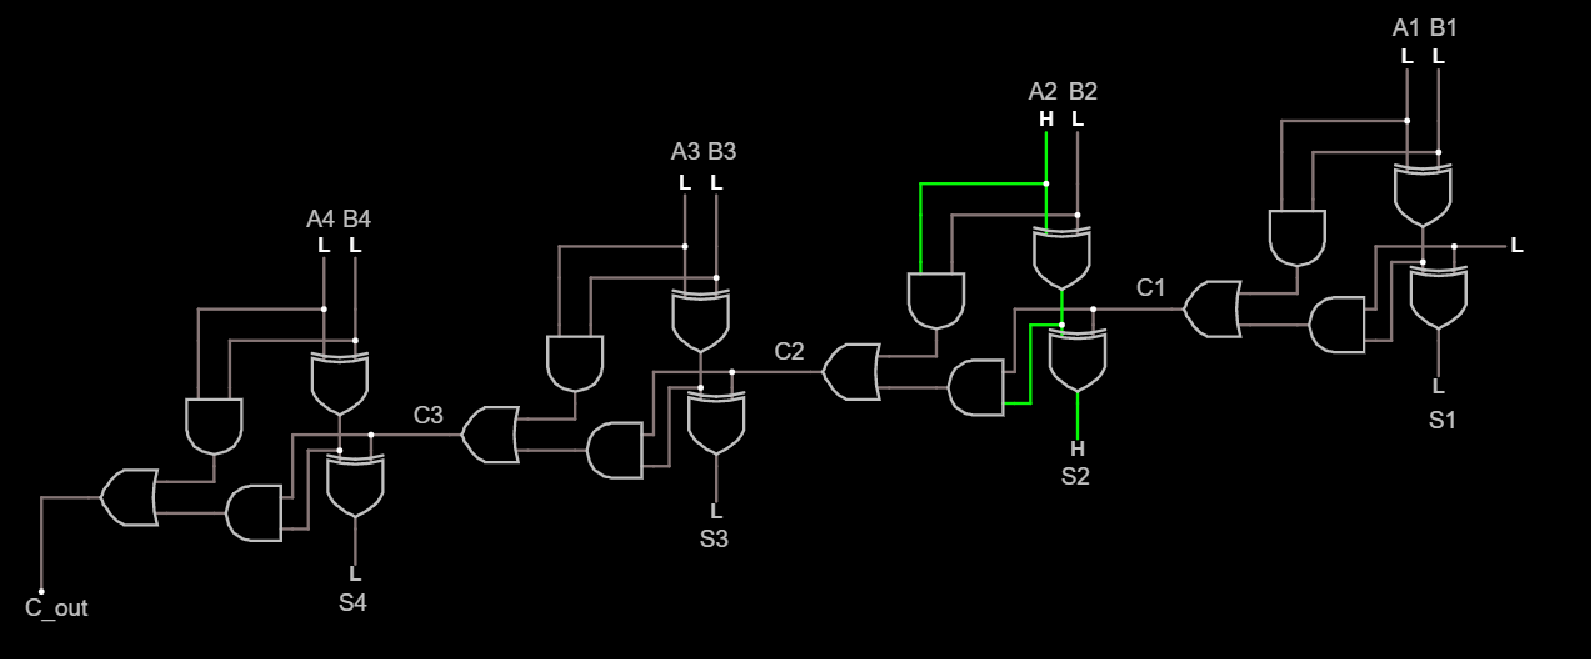
\includegraphics[width=\textwidth]{4bit/4bit_100.png}
		\end{subfigure}
		
		\begin{subfigure}[b]{0.8\textwidth}
			\centering
			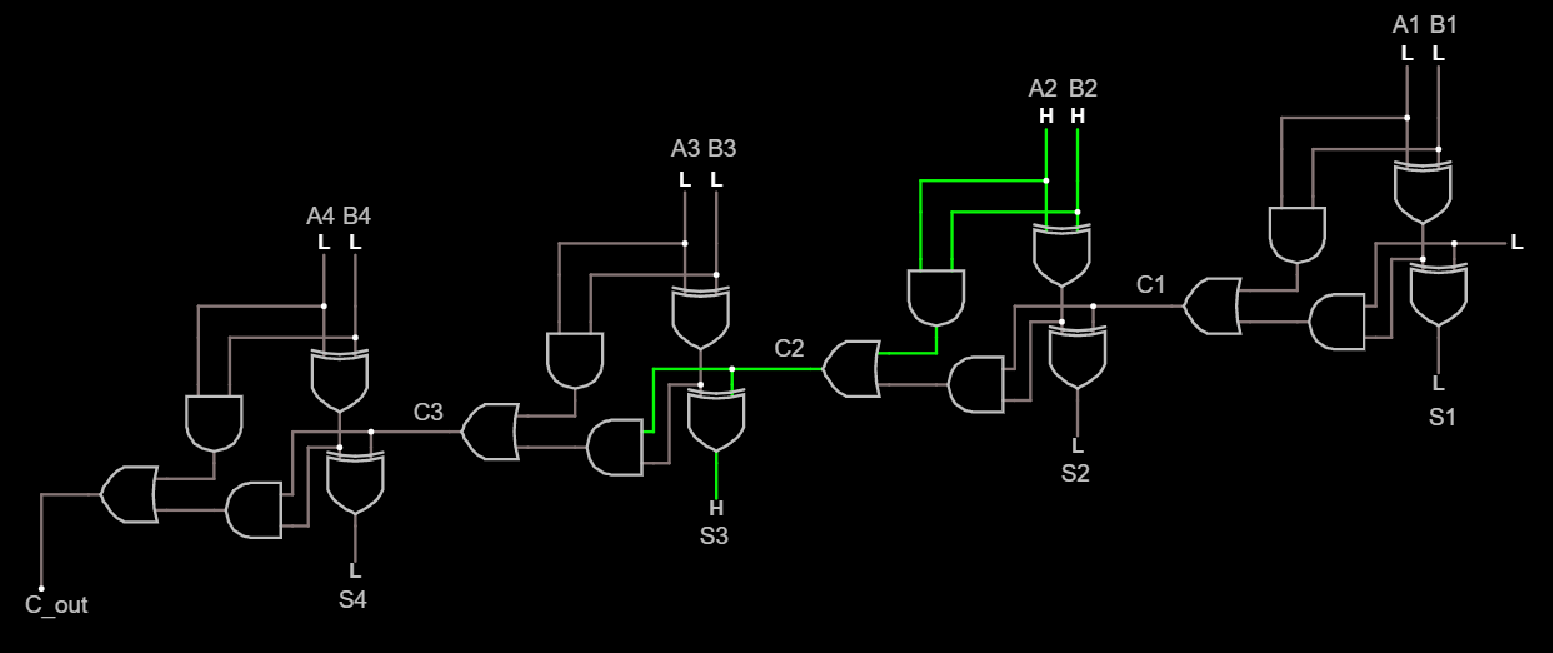
\includegraphics[width=\textwidth]{4bit/4bit_110.png}
		\end{subfigure}
	
		\caption{4-bit adder circuit}
		\label{4bit1}
	\end{figure}
	
	
	\begin{figure}
		\centering
		
		\begin{subfigure}[t]{.8\textwidth}
			\centering
			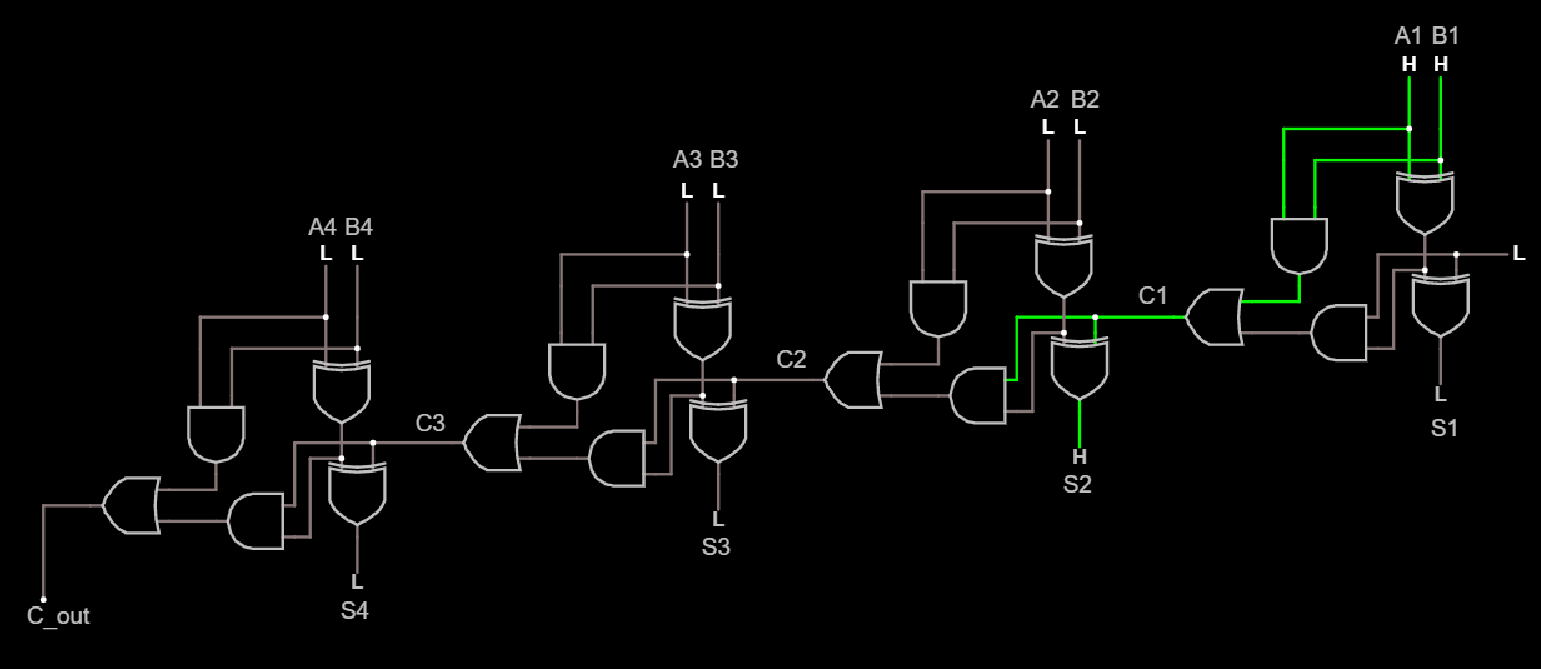
\includegraphics[width=\textwidth]{4bit/4bit_001.png}
		\end{subfigure}
	
		\begin{subfigure}[b]{0.8\textwidth}
			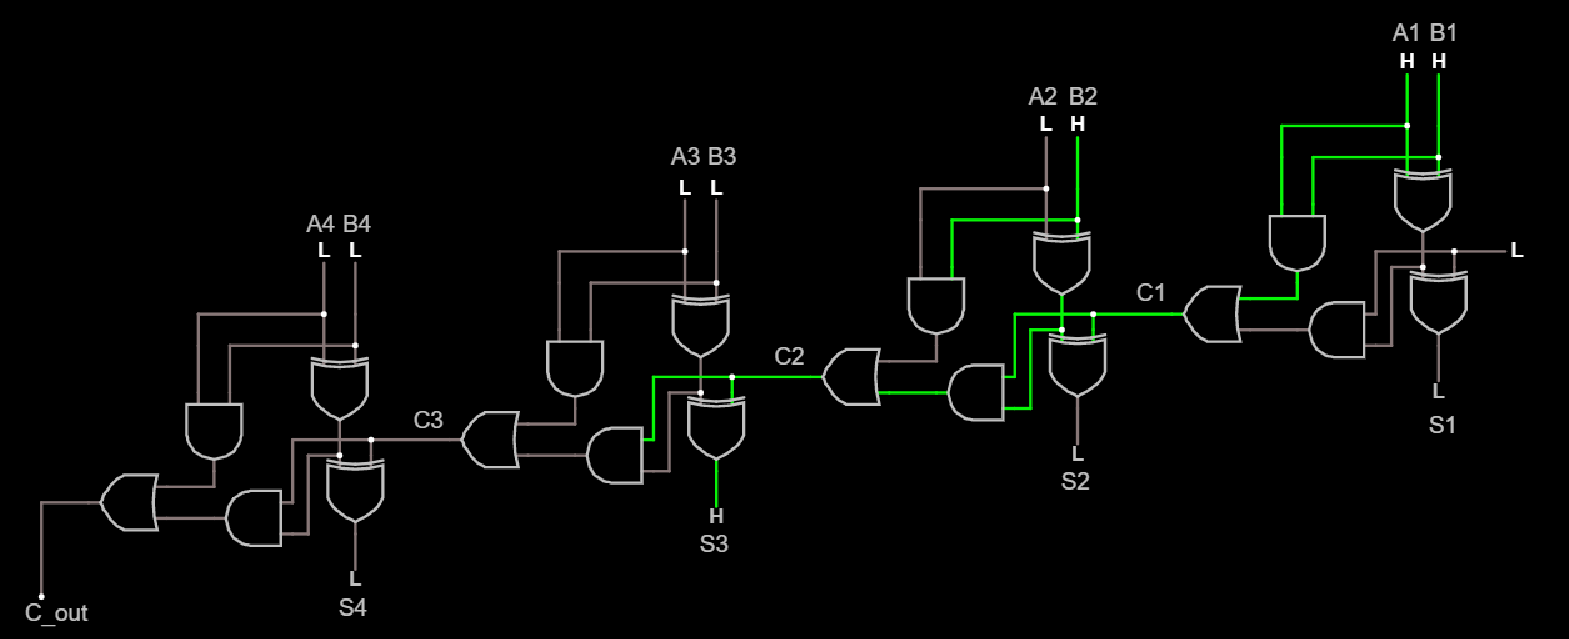
\includegraphics[width=\textwidth]{4bit/4bit_011.png}
		\end{subfigure}
	
		\begin{subfigure}[b]{0.8\textwidth}
			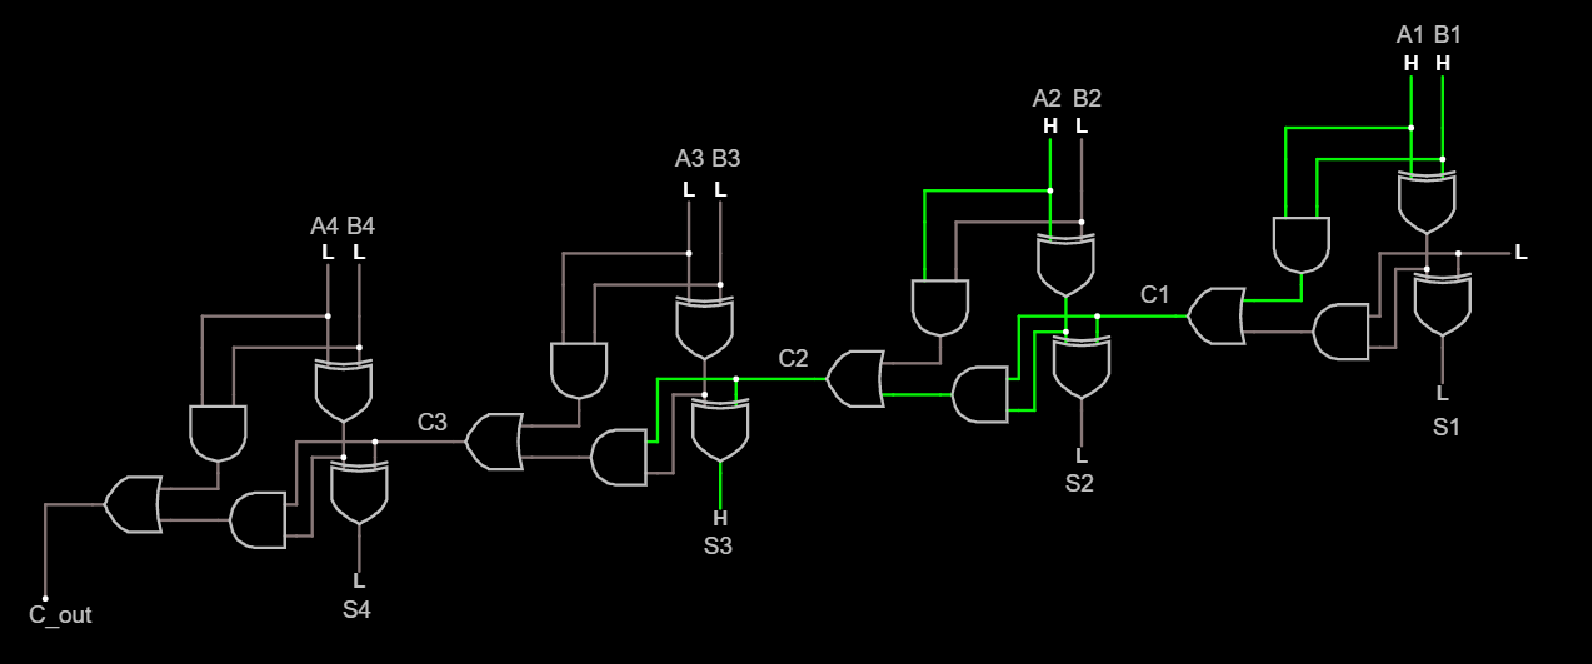
\includegraphics[width=\textwidth]{4bit/4bit_101.png}
		\end{subfigure}
		
		\begin{subfigure}[b]{0.8\textwidth}
			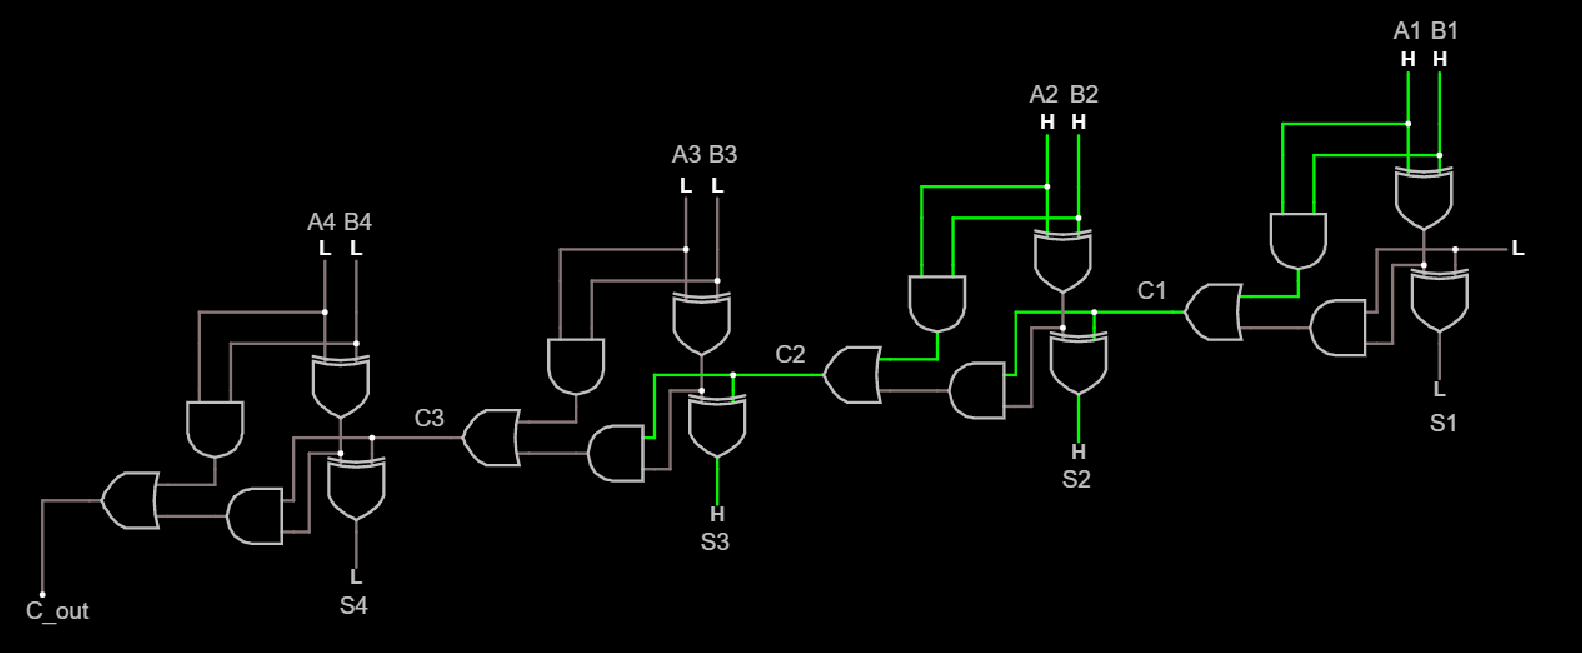
\includegraphics[width=\textwidth]{4bit/4bit_111.png}
		\end{subfigure}
		\caption{(Cont.) 4-bit adder circuit.}
		\label{4bit2}
	\end{figure}
\end{document}